\textbf{COLUNI 2022 -- Questão 27}\par\medskip Alguns métodos contraceptivos podem prevenir uma gravidez indesejada, como as pílulas contraceptivas orais, o diafragma e o DIU (Dispositivo Intra-Uterino), enquanto outros, como a camisinha masculina e a camisinha feminina, podem, além de evitar a fecundação, prevenir as IST´s (Infecções Sexualmente Transmissíveis). Existem ainda os métodos contraceptivos cirúrgicos, como a laqueadura e a vasectomia, que não previnem as IST’s, mas esterilizam, respectivamente, mulheres e homens que, dentro do planejamento familiar, não desejam mais ter filhos. A figura a seguir demonstra os locais de secção realizados na esterilização cirúrgica masculina.

\par

% COLUNI-AUTO-FIGURES-BEGIN
\begin{figure}[htbp]
\centering
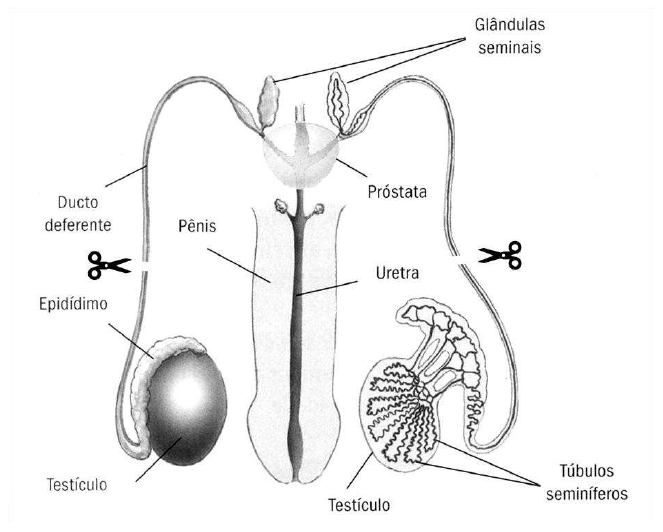
\includegraphics[width=0.95\linewidth]{static/simulados/coluni/figuras/2022/questao-27/figura-1.png}
\end{figure}
% COLUNI-AUTO-FIGURES-END

Esquema em corte e em vista frontal, mostrando os órgãos do sistema genital masculino. Os locais de secção da vasectomia estão indicados pelas tesouras (Elementos fora de proporção de tamanho entre si). Fonte: JUNIOR, C. S. \textit{et al.} Ciências entendendo a natureza, 8º ano. 24 ed. São Paulo. Ed. Saraiva. 2013. p. 227 (Adaptado).

\par

Com base na figura e em conhecimentos sobre a anatomia e a fisiologia do sistema genital masculino, é CORRETO afirmar que a eficácia da vasectomia se justifica:


\begin{enumerate}
\item por não ser mais possível a produção e a liberação de espermatozoides.
\item pela alteração na produção de hormônios sexuais masculinos.
\item por impedir a ejaculação e, consequentemente, a liberação de espermatozoides.
\item pela ausência de espermatozoides no sêmen.\end{enumerate}
